\section{Information Theory}
\subsection{Defining Information}

\noindent
 The following sections gets us thinking about how we might represent and encode information in a computer system.
 This slightly deals with probability, but we will not cover it in depth.
 \cite{terman2017computation_structures}.

\begin{Def}[Information]

    \label{def:info}

    \textbf{Information} measures the amount of uncertainty about a given fact provided some data.
\end{Def}

\begin{Example}[Playing Deck of Cards]

    \label{ex:card_info}

    Given a 52-card deck, a card is drawn at random. One of the following data points is revealed:
    \renewcommand{\labelenumi}{\alph{enumi})}
    \begin{enumerate}
        \item The card is a heart (13 possibilities).
        \item The card is not the Ace of Spades (51 possibilities).
        \item The card is the ``Suicide King,'' i.e., King of Hearts (1 possibility).
    \end{enumerate}

    \vspace{-1.5em}
\end{Example}

\begin{Def}[Quantifying Information]

    \label{def:quant_info}

    Given a discrete (finite) random variable $X$ with $n$ possible outcomes ($x_1, x_2, \ldots, x_n$) and a probability $P(X) = p_i$ for each outcome $x_i$, the \textbf{information content} of $X$ is defined as:
    \[
    I(X_i) := \log_2\left(\dfrac{1}{p_i}\right)
    \]
    \noindent
    Where $1/p_i$ is the probability of $x_i$, while Log base 2 measures how many bits (0 or 1) are needed to represent the outcome.
\end{Def}

\newpage 

\begin{Example}[Generalizing Information Content]

    \label{ex:card_info_content}

    A heart drawn from a 52-card deck may be represented as follows:
    \[I(\text{heart}) = \log_2\left(\dfrac{1}{13/52}\right) \approx 2 \text{ bits}\]

    \noindent
    More generally, we may redefine the information content as follows:

    \[
        I(\text{data}) = \log_2\left(\dfrac{1}{M \cdot (1/N)}\right) = \log_2 \left(\dfrac{N}{M}\right)
    \]

    \noindent
    Where $N$ is the total number of possible outcomes (e.g., 52 cards in a deck), and $M$ is the number of outcomes that match 
    the data (e.g., 13 hearts in a deck). Hence, $M\cdot (1/N)$ is the amount of information received from the data. Consider two more examples:
    \begin{itemize}
        \item \textbf{Information in one coin flip:} $\log_2\left(2/1\right) = 1$ bit ($N:=2, M:=1$).
        \item \textbf{Rolling 2 dice:} $\log_2\left(36/1\right) \approx 5.17$ or 6 bits ($N:=36, M:=1$).
    \end{itemize}
\end{Example}

\begin{Def}[Entropy]

    \label{def:entropy}

    The \textbf{entropy} of a discrete random variable $X$ is the average amount of information contained in all possible outcomes of $X$.
    It is defined as:
    \Large
    \[
    H(X) := E(I(X)) = \sum_{i=1}^{N} p_i \cdot \log_2\left(\dfrac{1}{p_i}\right)
    \]

    \normalsize
    \noindent
    Where function $E$ is the expected value (i.e., average) of the information content $I(X)$ across all outcomes of $X$.
    This conveys how many bits $b$ are needed to represent the outcomes of $X$:
    \begin{itemize}
        \item $b < H(X)$: Information is lost (i.e., not all outcomes can be represented).
        \item $b = H(X)$: An optimal representation.
        \item $b > H(X)$: Redundancy (i.e., not an efficient use of resources.).
    \end{itemize}
\end{Def}

\begin{Tip} For refreshers on $\sum$ consider our other text:
    \href{https://github.com/Concise-Works/Discrete-Math}{Concise Works: Discrete Math}.
\end{Tip}

\newpage 
\begin{Example}[The Entropy of Four Choices]

    \label{ex:entropy_four}

    Consider a discrete random variable and it's possible outcomes $X:=\{A,B,C,D\}$:

    \begin{center}
        
        \begin{tabular}{c c c}
          \toprule
          choice$_i$ & $p_i$ & $\log_2\bigl(1/p_i\bigr)$ \\
          \midrule
          A & $\displaystyle 1/3$  & $1.58\,\mathrm{bits}$ \\
          B & $\displaystyle 1/2$  & $1\,\mathrm{bit}$    \\
          C & $\displaystyle 1/12$ & $3.58\,\mathrm{bits}$ \\
          D & $\displaystyle 1/12$ & $3.58\,\mathrm{bits}$ \\
          \bottomrule
        \end{tabular}
    \end{center}

    \noindent
    Hence, the entropy of $X$ is:
    \begin{align*}
        H(X) := \sum_{i=1}^{4} p_i \cdot \log_2\left(\dfrac{1}{p_i}\right)= & \left(\dfrac{1}{3} \cdot 1.58\right) +\\
        &\left(\dfrac{1}{2} \cdot 1\right) +\\
        &\left(\dfrac{1}{12} \cdot 3.58\right) +\\
        &\left(\dfrac{1}{12} \cdot 3.58\right) +\\
        \approx &\ 1.626\,\mathrm{bits}
    \end{align*}

    \noindent 
    The entropy of $X$ is approximately 1.626 bits, meaning that on average, we should be able to represent the outcomes of $X$ 
    using less than 2 bits per outcome.

\end{Example}

\noindent
Let's discuss how we might go about representing our outcomes:
\begin{Def}[Encoding]

    \label{def:encoding}
    
        An \textbf{encoding} is an \underline{unambiguous} mapping from a set of symbols to a set of bit strings:
        \begin{itemize}
                \item \textbf{Fixed-length encoding:} Uses a fixed number of bits to represent each symbol.
                \item \textbf{Variable-length encoding:} Uses a different number of bits for each symbol.
        \end{itemize}
\end{Def}

\newpage 

\begin{Example}[Encoding Four Symbols]

    \label{ex:encoding_four}

    Consider the four symbols $A, B, C, D$ and each possible encoding for them:\\

    \noindent
    \begin{center}
   
  \begin{tabular}{c c c c c c}
    \toprule
    & \multicolumn{4}{c}{\textbf{Encoding for each symbol}} & \textbf{Encoding for,} \\
    &A & B & C & D & ``ABBA'' \\
    \midrule
    1.)&\texttt{00} & \texttt{01}  & \texttt{10}  & \texttt{11}  & \texttt{00 01 01 00} \\
    2.)&\texttt{01} & \texttt{1}   & \texttt{000} & \texttt{001} & \texttt{01 1 1 01}  \\
    3.)&\texttt{0}  & \texttt{1}   & \texttt{10}  & \texttt{11}  & \texttt{0 1 1 0}    \\
    \bottomrule
  \end{tabular}

    \end{center}

    \vspace{1em}
  \noindent
  (1) Is a fixed-length encoding, (2) is a variable-length encoding, and (3) is also a variable-length encoding and
  uses fewer bits; \textbf{However}, it is ambiguous. Depending on how our program reads the string, it may group and misinterpret 
  the bits.\\

  \noindent
  E.g., (3) could be, ``0 11 0'' (A D A) or `` 0 1 10'' (A B C). Hence, an invalid encoding.
\end{Example}

\begin{theo}[Binary Tree Encoding]

    \label{theo:binary_tree_encoding}

    Binary trees may represent unambiguous encodings, where each symbol is a leaf 
    node, and each edge represents the next bit. Since each path is unique, the encoding is unambiguous.
\end{theo}

\begin{figure}[ht!]

    \centering
    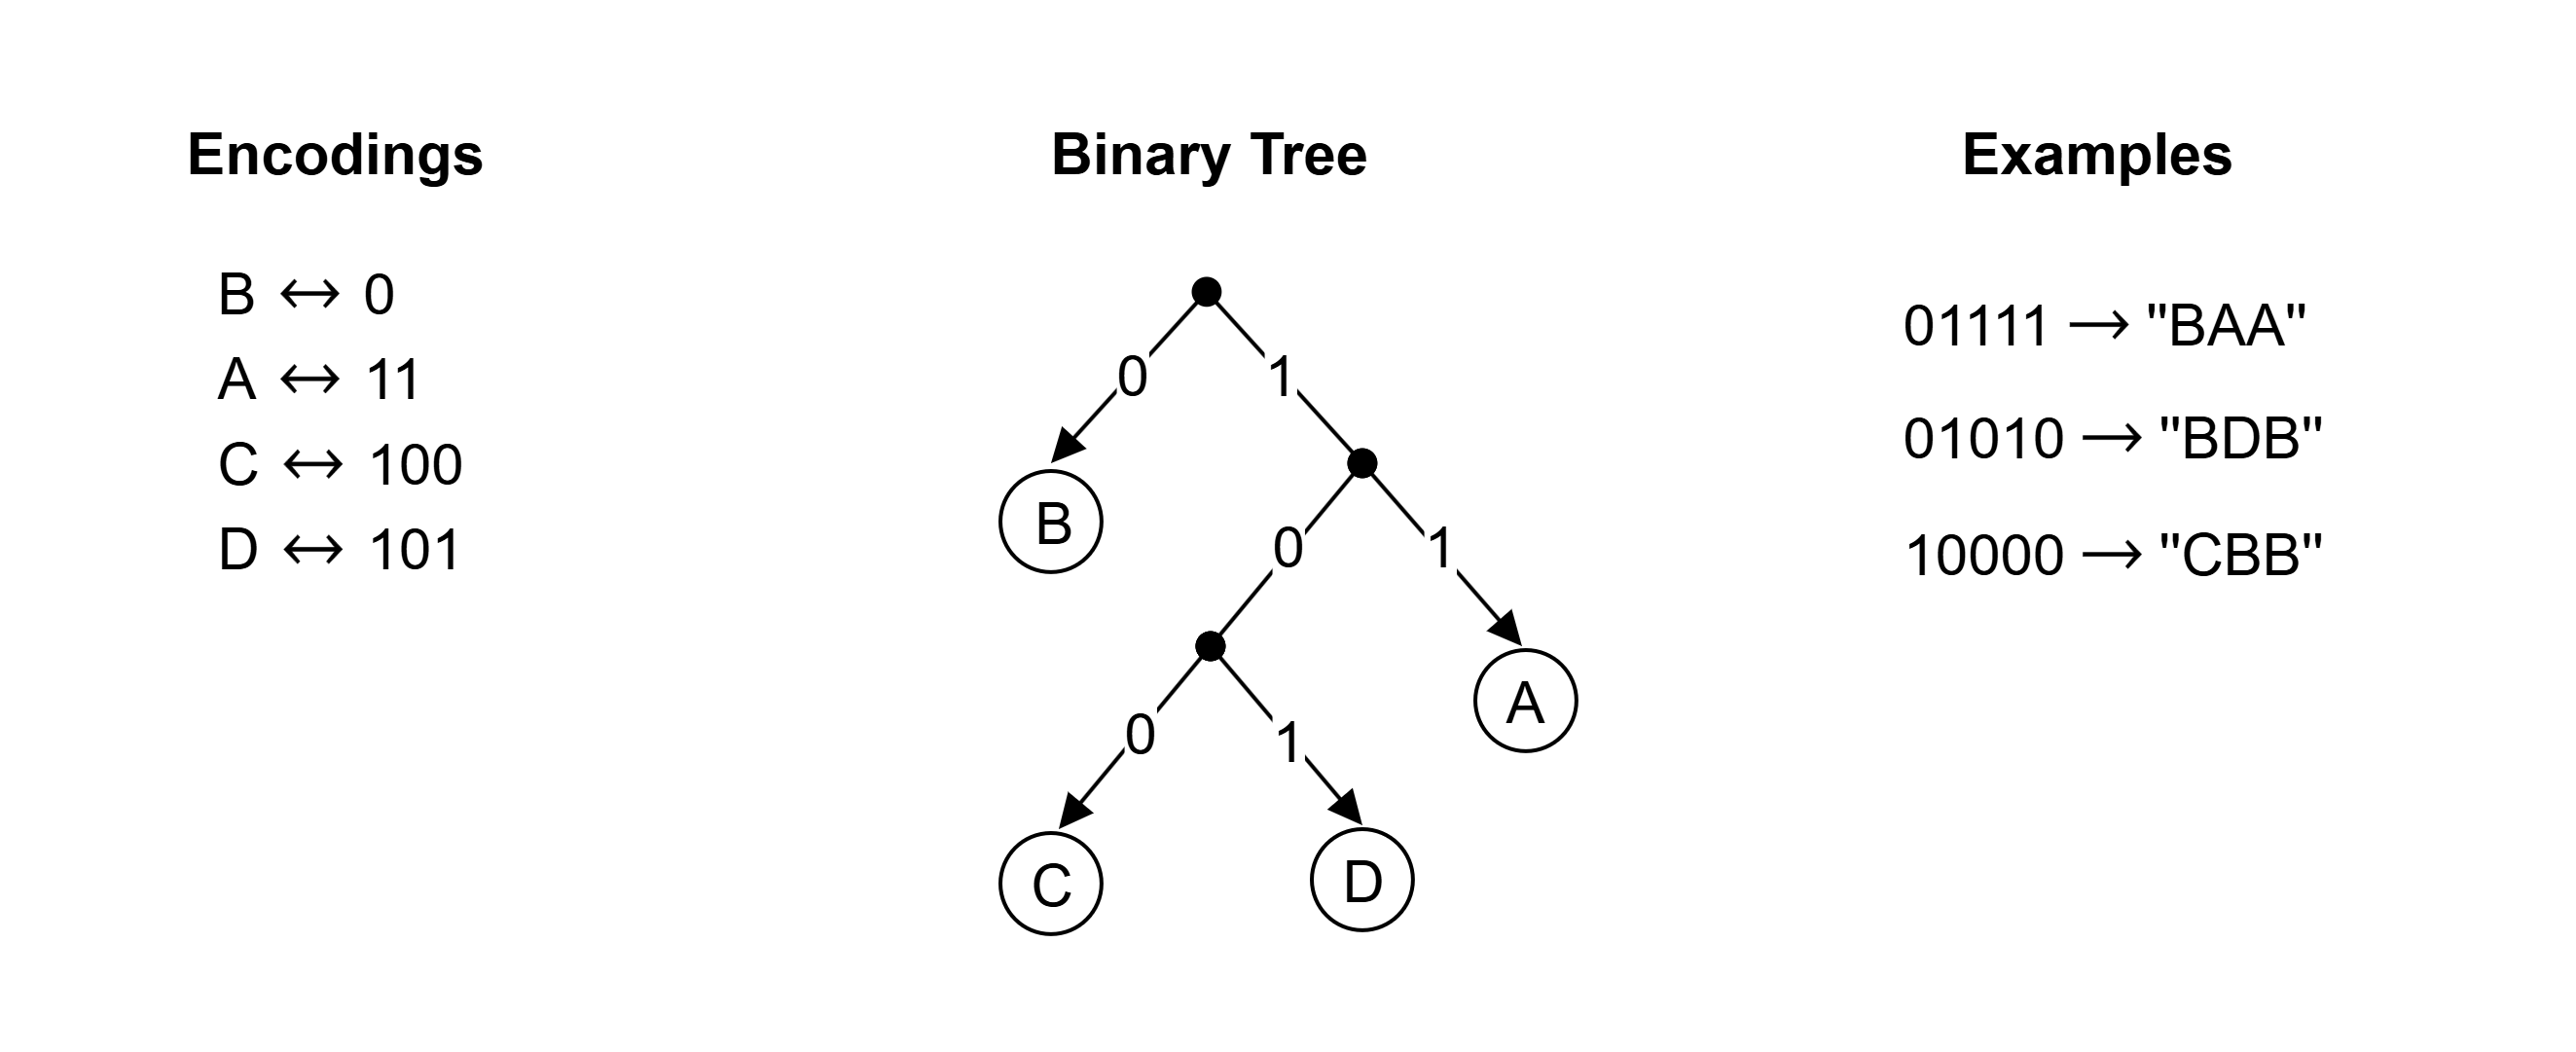
\includegraphics[width=\textwidth]{./Sections/comp/info/binary_tree_encoding.png}
    \caption{Encodings start at the root, each edge taken writes the next bit.}

    \label{fig:binary_tree_encoding}
\end{figure}

\newpage 
\noindent

\begin{theo}[Binary Tree Encoding -- Fixed-Length]

    \label{theo:fixed_length_encoding}

    \noindent
    A fixed-length encoding is optimal when the number of symbols $n$ bear an equal probability of occurrence. 
    In a binary tree encoding, all leaves have the same depth.\\

    \noindent
    I.e., for $n$ symbols, each have a probability of $1/n$, hence an entropy of:
    \[
    H(X) = \sum_{i=1}^{n} \left(\dfrac{1}{n} \cdot \log_2\left(\dfrac{1}{1/n}\right)\right) = \log_2(n)
    \]
\end{theo}

\begin{figure}[ht!]

    \centering
    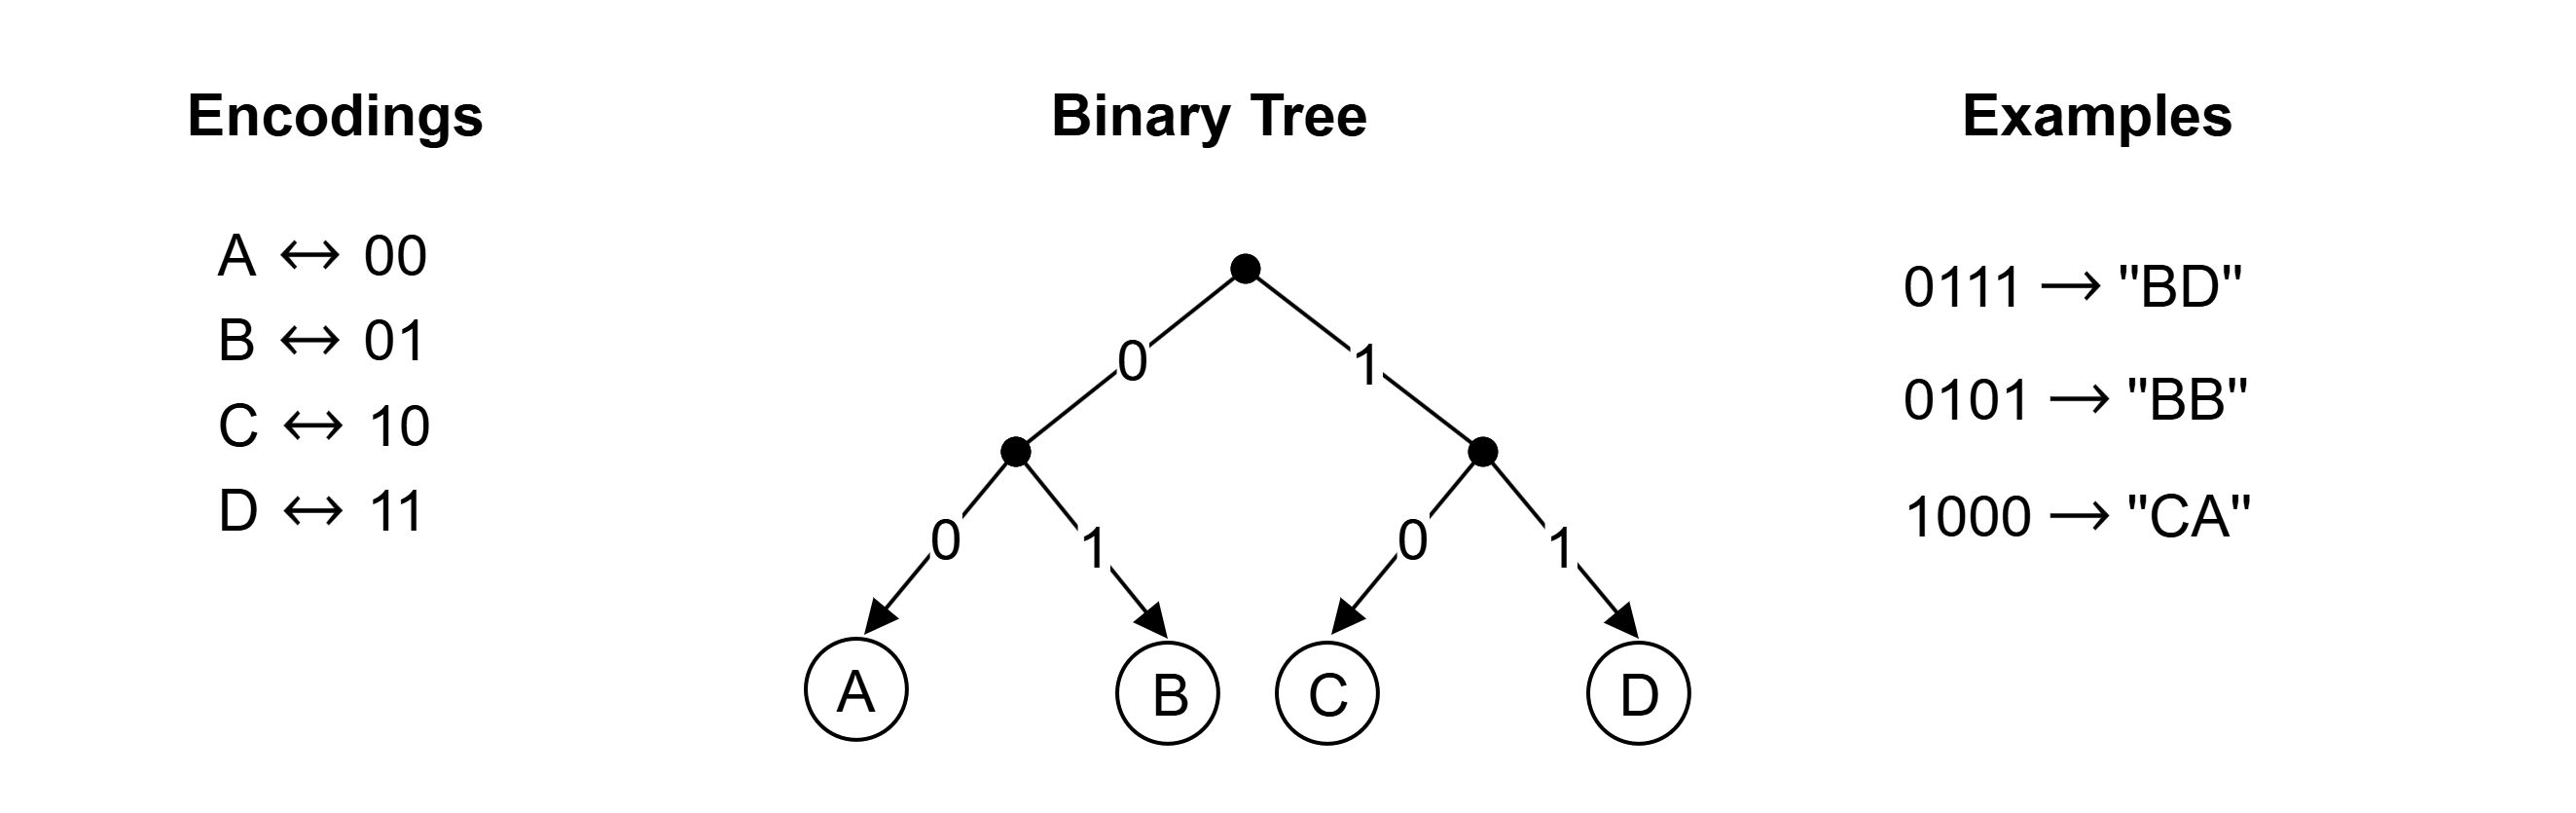
\includegraphics[width=\textwidth]{./Sections/comp/info/bt_fixed.png}
    \caption{A fixed-length encoding for four symbols, represented as a binary tree.}

    \label{fig:fixed_length_encoding}
\end{figure}

\begin{theo}[Choosing Variable-Length Encoding]

    \label{theo:variable_length_encoding}

    \noindent
    If a symbol $A$ has the high probability of occurrence, it should be represented with the shortest possible bit string.
    Vice versa, if symbol $B$ has the low probability, then it should receive the longest bit string.\\

    \noindent
    E.g., in Figure (\ref{fig:binary_tree_encoding}), the symbol $B$ may be assumed to have the highest probability of occurrence,
    with $C$ and $D$ having the lowest.
\end{theo}

\begin{theo}[Variable vs. Fixed-Length Encoding]

    \label{theo:variable_vs_fixed_length_encoding}

    \noindent
    Though we would like to use a variable-length encoding in theory, a fixed-length encoding for complex 
    data structures is provides simplicity and scalability.
\end{theo}

\noindent
Moving forward we focus on such fixed-length encodings.

\newpage 



